\section{Erstellte Werkzeuge und Code-Bibliotheken}
\label{sec:recorder}
In dieser Arbeit mussten viele Features und Konfigurationen der Entscheidungsbäume untersucht und zu getestet werden. Aus diesem Grund wurde eine umfangreiche Infrastruktur in Rust und Python geschaffen,
die die Auswertung von ML Modellen mit den Handgestendaten vereinfacht. Die Infrastruktur umfasst ein Datenmodel für Handgesten und kann die Datenmengen mit verschiedenen Parsing-Methoden einlesen.
Außerdem können synthetischen Daten auf verschiedene Arten generiert werden. Abbildung \ref{fig:architecture_overview} zeigt ein Abhängigkeitsdiagramm der einzelnen Module.
Alle Funktionalitäten wurden in Code-Bibliotheken extrahiert, um die Integration in Hilfsprogramme zu vereinfachen.
\begin{figure}
    \centering
    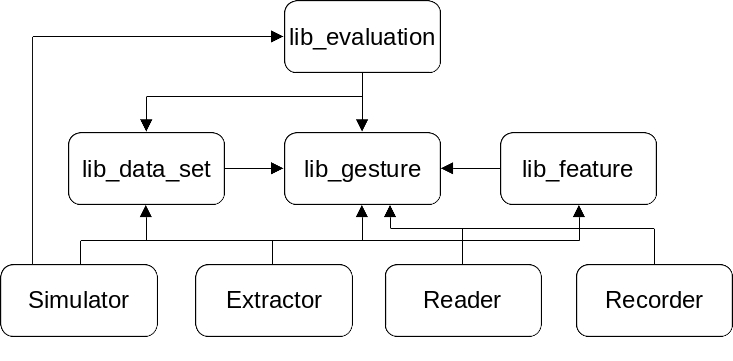
\includegraphics[width=0.75\linewidth]{images/architecture_overview.jpg}
    \caption{Abhängigkeitein der einzelnen Module.}
    \label{fig:architecture_overview}
\end{figure}
\newline
\newline
\texttt{lib\_gesture} definiert die Handgeste und die vorhandenen Handgestentypen. Außerdem implementiert sie zwei Parsing-Methoden. Die erste Methode parsed Handgesten nach Annotation und die
zweite nach Kubiks Algorithmus (Kapitel \ref{sec:gesture_extraction}). Die Handgeste implementiert Methoden, um synthetische Daten zu generieren.
\begin{itemize}
    \item Rotation um 90°, 180° und 270°.
    \item Nullgesten durch Kombination der ersten Hälfte der Ausgangshandgeste und der zweiten Hälfte von dessen Rotationen.
    \item Verschiebung um einen Pixel nach oben und unten für eine Handgeste von links nach rechts bzw. rechts nach links und analog eine Verschiebung nach links und rechts für eine Handgeste von oben nach unten bzw.
    unten nach oben.
    \item Rotation der äußeren Pixel, um diagonale Handgesten zu generieren.
\end{itemize}
\texttt{lib\_feature} bietet ein einfaches Interface an, um Features aus einer Handgeste zu implementieren. Listing \ref{lst:FeatureInterface} beschreibt das Interface in Rust. Ein Feature kann aus einer
Handgeste berechnet werden und deserialisiert werden. Zurzeit sind 30 verschiedene Variationen an Features implementiert (Tabelle \ref{tab:implemented_features}).
\begin{lstlisting}[label=lst:FeatureInterface,caption={Das Interface, um ein Feature zu implementieren.}]
pub trait Feature {
    fn calculate(gesture: &Gesture) -> Self where Self: Sized;
    fn marshal(&self) -> String;
}
\end{lstlisting}
\begin{table}[h!]
    \centering
    \begin{tabular}{ | p{0.3\linewidth} | p{0.7\linewidth} | }
        \hline
        Feature & Variation \\\hline
        Helligkeitsverteilung & Minimum/Maximum über alle Zeitfenster \\\hline
        Helligkeitsverteilung & Geometrisches Minimum/Maximum \\\hline
        Helligkeitsverteilung & Quadranten mit Minima/Maxima \\\hline
        Helligkeitsverteilung & Minima/Maxima Zeilenweise über 3 und 6 Zeitfenster \\\hline
        Helligkeitsverteilung & Minima/Maxima Spaltenweise über 3 und 6 Zeitfenster \\\hline
        Schwerpunktverteilung & Mit Ganzzahlen in horizontaler und vertikaler Richtung \\\hline
        Schwerpunktverteilung & Mit Fließkommazahlen in horizontaler und vertikaler Richtung \\\hline
        Motion History Image & 8-Bit und 16-Bit \\\hline
        Standardabweichung & - \\\hline
        Durchschnitt & - \\\hline
        Maximum/Minimum & - \\\hline
        Summe der Gradienten & Von Frame zu Frame \\\hline
        Summe der Gradienten & Von benachbarten Pixel in Spaltenweise und Zeilenweise \\\hline
        Summe der Gradienten & Spaltenweise und Zeilenweise Summe der Gradienten zusammengefasst pro Zeitfenster \\\hline
        Durchschnittliche Änderung der Amplitude & - \\
        \hline
    \end{tabular}
    \caption{Implementierte Features in \texttt{lib\_feature}.}
    \label{tab:implemented_features}
\end{table}
\texttt{lib\_data\_set} stellt alle Trainings- und Testmengen, die im Laufe dieser Fallstudie aufgenommen wurden, als statische Importe bereit. Einträge sind bereits nach Distanz zur Kamera,
Helligkeit, Verdeckungsobjekt (Hand und Finger) und Ausführungsgeschwindigkeit sortiert. Die Helligkeit eines Eintrags kann durch einen statischen Offset verändert werden, sodass die Helligkeit jedes
Pixels um den Offset erhöht oder verringert wird, oder durch eine Skalierung verändert werden.
\newline
\newline
\texttt{lib\_evaluation} bietet ein Hilfsobjekt an, dass Datenmengen nach Klassifizierungsgenauigkeit auswertet und Berichte daraus generiert.
\newline
\newline
Der \texttt{Simulator} ist zweigeteilt. Ein Teil nutzt die Gestenkandidatenerkennungsmethode nach Kubik, die in \texttt{lib\_gesture} implementiert ist, um den seriellen Datenstrom von der Kamera in
Echtzeit zu verarbeiten. Wenn ein Gestenkandidat gefunden wird, wird er durch das hinterlegte Modell klassifiziert. Das Ergebnis wird auf der Konsole ausgegeben. Der andere Teil evaluiert
Testmengen aus der Bibliothek \texttt{lib\_data\_set} mit dem hinterlegten Modell und gibt Statistiken zu der Klassifizierungsgenauigkeit auf der Konsole aus.
\newline
\newline
Der \texttt{Extractor} extrahiert aus spezifizierten Datenmengen alle definierten Features und exportiert diese in Dateien. Die können bei der Konstruktion eines Modells eingelesen werden und zum Trainieren
genutzt werden. Optional kann die Datenmenge durch synthetische Daten erweitert werden.
\newline
\newline
Der \texttt{Reader} gibt den seriellen Datenstrom von der Kamera auf der Konsole aus. Dies kann zum Fehler finden und Testen der programmierten Firmware genutzt werden.
\newline
\newline
Der \texttt{Recorder} nutzt, wie der \texttt{Simulator}, den seriellen Datenstrom der Kamera und die Parsing-Methode von Kubik, um Gestenkandidaten zu erkennen.
Der Gestenkandidat wird dann in eine vordefinierte Datei geschrieben. Es gibt drei Aufnahmemechanismen, um effizient annotierte Trainings- und Testmengen aufzunehmen.
\begin{enumerate}
    \item Es wird immer zwischen dem ausgewählten Handgestentypen und seinem inversen Handgestentypen hin und her gewechselt. Dieser Ansatz wurde von Kubik vorgeschlagen \cite{venzkeArticle}.
    \item Es kann ein fixer Handgestentyp ausgewählt werden, mit dem alle Gestenkandidaten beschriftet werden.
    \item Jedes Mal, wenn ein Gestenkandidat erkannt wurde, wird erfragt welcher Handgestentyp es ist.
\end{enumerate}